\resizebox{\textwidth}{!}{%
      \centering
    \scriptsize
    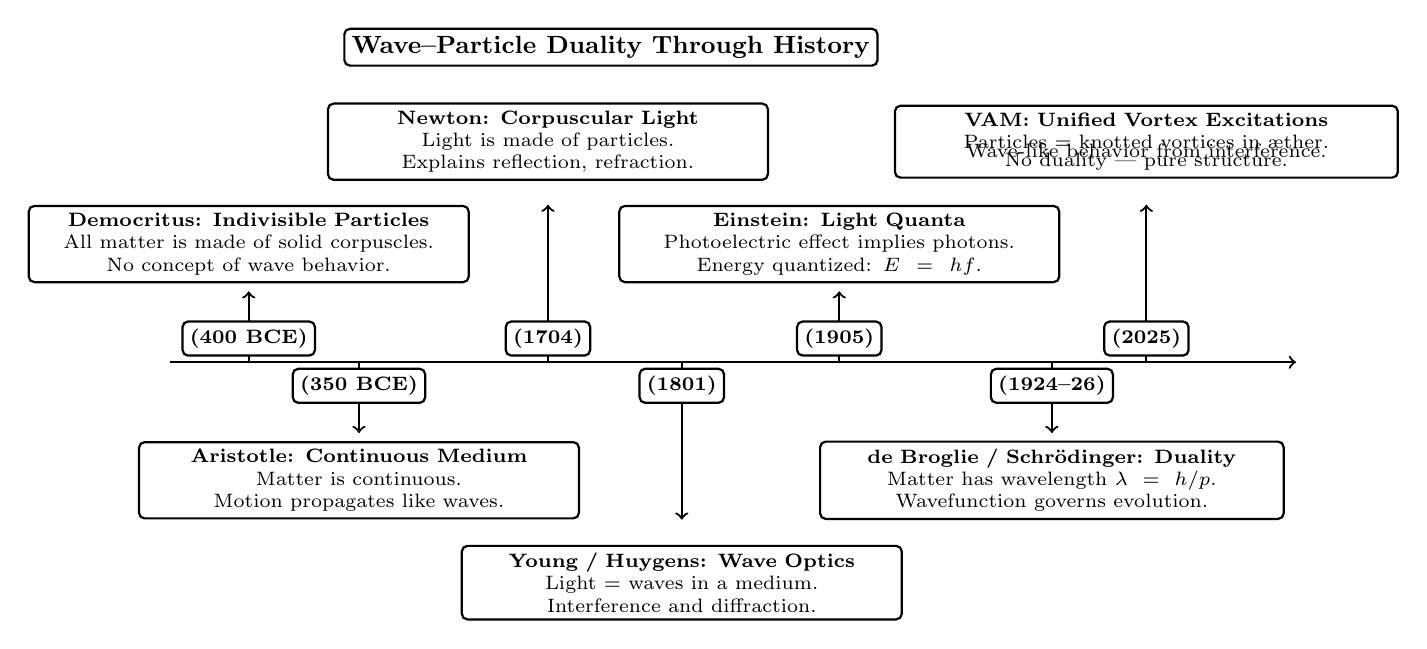
\begin{tikzpicture}
    \scriptsize

    % Timeline base
    \draw[->, thick] (-1,0) -- (13.3,0);

    % Arrows above timeline
    \draw[->, thick] (0,0) -- (0,0.9);       % Democritus
    \draw[->, thick] (3.8,0) -- (3.8,2.0);   % Newton
    \draw[->, thick] (7.5,0) -- (7.5,0.9);   % Einstein
    \draw[->, thick] (11.4,0) -- (11.4,2.0); % VAM

    % Arrows below timeline
    \draw[->, thick] (1.4,0) -- (1.4,-0.9);     % Aristotle
    \draw[->, thick] (5.5,0) -- (5.5,-2.0);     % Young/Huygens
    \draw[->, thick] (10.2,0) -- (10.2,-0.9);   % de Broglie

    % --- Date labels ---
    \node[draw, thick, rounded corners=2pt, fill=white, align=center, font=\bfseries ] at (0, .3)   {(400 BCE)};
    \node[draw, thick, rounded corners=2pt, fill=white, align=center, font=\bfseries ] at (3.8, .3) {(1704)};
    \node[draw, thick, rounded corners=2pt, fill=white, align=center, font=\bfseries ] at (7.5, .3) {(1905)};
    \node[draw, thick, rounded corners=2pt, fill=white, align=center, font=\bfseries ] at (11.4, .3){(2025)};

    \node[draw, thick, rounded corners=2pt, fill=white, align=center, font=\bfseries ] at (1.4,- .3) {(350 BCE)};
    \node[draw, thick, rounded corners=2pt, fill=white, align=center, font=\bfseries ] at (5.5,- .3) {(1801)};
    \node[draw, thick, rounded corners=2pt, fill=white, align=center, font=\bfseries ] at (10.2,- .3) {(1924--26)};

    % Timeline label
    \node[draw, thick, fill=white, rounded corners=2pt, font=\small] at (4.6,4.0) {\textbf{Wave–Particle Duality Through History}};

    % --- Democritus ---
    \node[draw, rounded corners=2pt, thick, align=center, fill=white, text width=5.4cm] at (0,1.5) {
    \textbf{Democritus: Indivisible Particles} \\% [-0.8em]
    All matter is made of solid corpuscles. \\% [-0.8em]
    No concept of wave behavior.
    };

    % --- Newton ---
    \node[draw, rounded corners=2pt, thick, align=center, fill=white, text width=5.4cm] at (3.8,2.8) {
    \textbf{Newton: Corpuscular Light} \\% [-0.8em]
    Light is made of particles. \\% [-0.8em]
    Explains reflection, refraction.
    };

    % --- Einstein ---
    \node[draw, rounded corners=2pt, thick, align=center, fill=white, text width=5.4cm] at (7.5,1.5) {
    \textbf{Einstein: Light Quanta} \\% [-0.8em]
    Photoelectric effect implies photons. \\% [-0.8em]
    Energy quantized: \( E = hf \).
    };

    % --- VAM ---
    \node[draw, rounded corners=2pt, thick, align=center, fill=white, text width=6.2cm] at (11.4,2.8) {
    \textbf{VAM: Unified Vortex Excitations} \\% [-0.8em]
    Particles = knotted vortices in æther. \\[-0.6em]
    Wave-like behavior from interference. \\[-0.6em]
    No duality — pure structure.
    };

    % --- Aristotle ---
    \node[draw, rounded corners=2pt, thick, align=center, fill=white, text width=5.4cm] at (1.4,-1.5) {
    \textbf{Aristotle: Continuous Medium} \\% [-0.8em]
    Matter is continuous. \\% [-0.8em]
    Motion propagates like waves.
    };

    % --- Young / Huygens ---
    \node[draw, rounded corners=2pt, thick, align=center, fill=white, text width=5.4cm] at (5.5,-2.8) {
    \textbf{Young / Huygens: Wave Optics} \\% [-0.8em]
    Light = waves in a medium. \\% [-0.8em]
    Interference and diffraction.
    };

    % --- de Broglie / Schrödinger ---
    \node[draw, rounded corners=2pt, thick, align=center, fill=white, text width=5.7cm] at (10.2,-1.5) {
    \textbf{de Broglie / Schrödinger: Duality} \\% [-0.8em]
    Matter has wavelength \( \lambda = h/p \). \\% [-0.8em]
    Wavefunction governs evolution.
    };

    \end{tikzpicture}
    \caption{\textbf{Intellectual trajectory of wave–particle duality:} from classical corpuscles and wave models to quantum dualities and beyond. VAM reframes the dichotomy by modeling all excitations as topologically structured vortices in a fluid æther. In this view, “particles” and “waves” are unified as geometric flow phenomena—dispensing with dualism in favor of pure structure.}\label{fig:WaveParticleDuality}
}